\documentclass[border=10pt]{standalone}
\usepackage[utf8]{inputenc}
\usepackage[usenames,dvipsnames]{xcolor}
\definecolor{babyblue}{rgb}{0.54, 0.81, 0.94}
\definecolor{babypink}{rgb}{0.96, 0.76, 0.76}
\definecolor{blue(ncs)}{rgb}{0.0, 0.53, 0.74}
\definecolor{pistachio}{rgb}{0.58, 0.77, 0.45}
\definecolor{darksalmon}{rgb}{0.91, 0.59, 0.48}
\definecolor{lightsalmonpink}{rgb}{1.0, 0.6, 0.6}
\definecolor{columbiablue}{rgb}{0.61, 0.87, 1.0}
\definecolor{corn}{rgb}{0.98, 0.93, 0.36}
\definecolor{jonquil}{rgb}{0.98, 0.85, 0.37}
\definecolor{bananayellow}{rgb}{1.0, 0.88, 0.21}
\definecolor{blue(ncs)}{rgb}{0.0, 0.53, 0.74}
\title{plot}
\author{asabir}
\date{November 2021}
% from overleaf website 
\renewcommand*{\familydefault}{\sfdefault}
\usepackage{tikz}
\usepackage{pgfplots}
\begin{document}
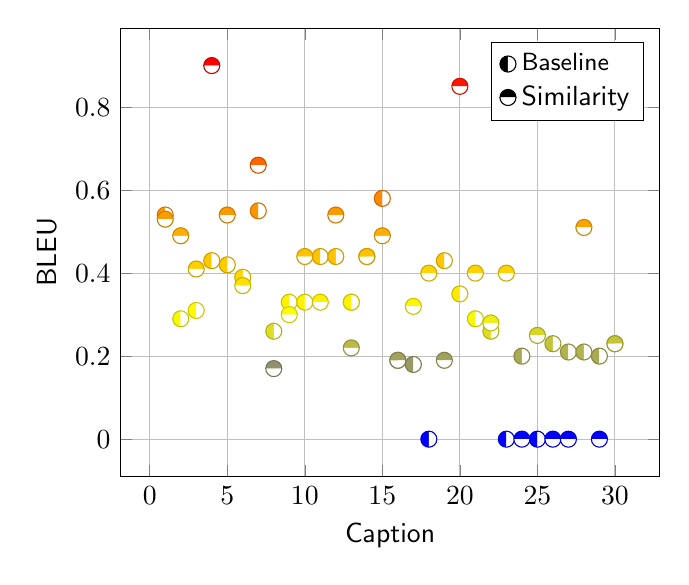
\begin{tikzpicture}
    \begin{axis}[
    %legend pos=south east,
    legend pos=north east,
    %legend pos=outer north east
grid=major,
       % legend
%yticklabel=\empty,
%legend pos=outer north east,
legend cell align={left}, % all 
        grid,
        %legend style={fill=none},
        %xlabel=\textsc{Re-ranked caption},
        xlabel=Caption,
        ylabel=  BLEU, 
       % legend style={
        %    at={(0.5,0.96)},
        %    anchor=west,
        %    mark size=1pt,
        %    legend columns=-1,
           % /tikz/every even column/.append style={column sep=0.cm}
         %   every node near coord/.append style={font=\tiny}Sim
        %},
    ]

%    \axispath\draw
   %         (7.49165,-10.02171)
%        |-  (8.31801,-11.32467)
%        node[near start,left] {$\frac{dy}{dx} = -1.58$};

%\addplot [blue!30, smooth,mark=*, line width=0.5mm] coordinates {
\addplot [only marks,
    scatter,
    mark=halfcircle*,
   %mark=triangle*,
    mark options={rotate=90},
    mark size=2.9pt] coordinates {
%\addplot [scatter, mark=*, mark size=3pt, line width=2pt, mesh] coordinates {
      %\addplot [draw=none, fill=pistachio!40] coordinates {
% B1 beam
(1, 0.54)
(2, 0.29)
(3, 0.31)
(4, 0.43)
(5, 0.42)
(6, 0.39)
(7, 0.55)
(8, 0.26)
(9, 0.33)
(10,0.33)
(11,0.44)
(12,0.44)
(13,0.33)
(13,0.33)
(14, 0.44)
(15, 0.58)
(16,0.19)
(17, 0.18)
(18, 0)
(19, 0.43)
(20, 0.35)
(21, 0.29)
(22, 0.26)
(23, 0)
(24, 0.20)
(25, 0)
(26,0.23)
(27, 0.21)
(28, 0.21)
(29, 0.20)
(30, 0.23)
%(31, 0.44)
%(32, 0) 
%(1, 0.88)
%(2, 0.88)
%(3, 0.89)
%(4, 0.89)
%(5, 0.9)
%(6, 0.94)
%(7, 0.94)
%(8, 0.88)
%(9, 0.88)
%(10, 0.94)
%(11, 0.93)
%(12, 0.91)
%(13, 0.89)
%(14, 0.88)
%(15, 0.93)
%(16, 0.97)
%(17, 0.83)
%(18. 0.88)
%(19,0.88)
    };
%darksalmon!50
%\addplot [darksalmon!90,  smooth, mark=square*, line width=0.5mm]  coordinates {
\addplot [only marks,
    scatter,
    mark=halfcircle*,
    mark size=2.9pt] coordinates {

(1, 0.53)
(2, 0.49)
(3, 0.41)
(4, 0.90)
(5, 0.54)
(6, 0.37)
(7, 0.66)
(8, 0.17)
(9, 0.30)
(10,0.44)
(11, 0.33)
(12, 0.54)
(13, 0.22)
(14, 0.44)
(15, 0.49)
(16, 0.19)
(17, 0.32)
(18, 0.40)
(19, 0.19)
(20, 0.85)
(21, 0.40)
(22, 0.28)
(23, 0.40)
(24, 0)
(25, 0.25)
(26, 0)
(27, 0)
(28, 0.51)
(29,0)
(30, 0.23)
%(31, 0.33)
%(32, 0)


  %  \addplot plot coordinates {
%   SBERT-sts


%(1, 0.27)
%(2, 0.58)
%(3, 0.03)
%(4, 0.76)
%(5, 0.73)
%(6, 0.57)
%(7, 0.98)
%(8, 0.80)
%(9, 0.80)
%(10, 0.44)
%(11, 0.78)
%(12, 0.57)
%(13, 0.69)
%(14, 0.69)
%(15, 0.75)
%(16, 0.47)
%(17, 0.81)
%%(18, 0.90)
%%(19, 0.20)
    };
    
        \addplot [black!30,  smooth,  line width=0.8mm] coordinates {
%    %\addplot [blue(ncs)!20, line width=1mm] coordinates {
%    (1,0.40)
%(2, 0.18)
%(3, 0)
%(4, 0.43)
%(5, 0.35)
%(6, 0.29)
%(7, 0.26)
%(8, 0)
%(9, 0.20)
%(10, 0)
%(11,0.23)
%(11, 0.21)
%(12, 0.21)
%(13, 0.20)
%(14, 0.23)
%(15, 0.44)
%(16, 0) 
%(1, 0.53)
%(2, 0.49)
%(3, 0.37)
%(4, 0.66)
%(5, 0.44)
%(6, 0.54)
%(7,0.22)
%(8, 0.17)
%(9, 0.33) %
%(10,0.44)
%(11, 0.19)
%(12, 0.54)
%(13,0.30)
%(14, 0.90) 
%(15, 0.49) 
%(16, 0.53) 
%(17, 0.45)


};




%\addplot [green!20, mark=+,  line width=0.8mm]  coordinates {

%(1,0.26)
%(2, 0.23)
%(3, 0.15)
%(4, 0.95)
%(6, 0.25)
%(7, 0.25)
%(8, 0.24)
%(9, 0.10)
%(10, 0.17)
%(11, 0.12)
%(12, 0.18)
%(13, 0.31)
%(14,0.18)
%(15, 0.25)
%(16, 0.25)
%};

    %\addplot plot coordinates {
\addplot +[darksalmon!50,  line width=0.8mm] coordinates {
%    \addplot [blue(ncs)!20, line width=1mm] coordinates {
    
%(1, 0.32)
%(2, 0.40)
%(3, 0.19)
%(4, 0.85)
%(5, 0.40)
%(6, 0.28)
%(7, 0.40)
%(8, 0)
%(9, 0.25)
%(10, 0)
%(11, 0)
%(12, 0.51)
%(13,0)
%(14, 0.23)
%(15, 0.33)
%(16, 0)
%(1, 0.40)
%(2, 0.33)
%(3, 0)
%(4, 0.16)
%(5, 0.85)
%(6, 0.50)
%(7, 0.667)
%(8, 0.667)
%(9, 0.99)
%(10, 0.87)
%(11, 0.50)
%(12, 0.25)
%(13, 0.12)
%(14, 0.99)
%(15, 0.62)
%(16, 0.33)
%(17, 0.99)
%(18, 0.87)
%(19, 0.99)
    };
    
   % BLEU

\legend{ \small Baseline \\ Similarity\\}
    \end{axis}
\end{tikzpicture}
\end{document}
